\documentclass[12pt,nofootinbib]{revtex4}
%\documentclass[9pt,twocolumn]{article}
\usepackage{graphicx}
\usepackage{rotating}
\usepackage{ragged2e}
\usepackage{array}
\usepackage{amsmath}
\usepackage{multirow}
\usepackage{listings}
\setlength{\textwidth}{17cm}
\setlength{\textheight}{23.5cm}
\setlength{\topmargin}{-2.0cm}
\setlength{\oddsidemargin}{-0.5cm}
%\renewcommand{\baselinestretch}{1.5}

\usepackage{epstopdf}
%\usepackage{subfig}


%\DeclareGraphicsExtensions{.pdf}


\begin{document}

\section{Computational details}
The nucleobases (uracil, cytosine, thymine, adenine, guanine) were optimized at the MP2/aug-cc-pVTZ level, while the thymine-thymine $\pi$-stack dimer (T-T ST1) was optimized at the DFT with the dispersion correction level, $\omega$B97X-D3/6-31+G**. RI-MP2/cc-pVTZ geometries of A=T WC and G$\equiv$C Watson-Crick (WC) dimers were taken from 
the JSCH-2005 set,\cite{Hobza:bench:06} RI-MP2/cc-pVTZ geometry of the HBDI$^{-}$ chromophore was adapted from.\cite{Bravaya:NAB:10} $Trans$-polyenes employed in the numerical size-extensivity test were optimized at the RI-MP2/cc-pVTZ and RI-MP2/6-31G** levels for the calculations of ionization potentials with corresponding basis sets.

Equation-of-motion (EOM) coupled cluster with singles and doubles (CCSD), MP2T and MP2 ionization potential calculations were performed with the aug-cc-pVTZ basis for nucleobases, cc-pVTZ for dimers, cc-pVTZ and 6-31G** for the numerical size-extensivity tests with the $trans$-polyenes. All calculations were performed using Q-Chem 4.4 package.\cite{qchem_2014s}

\section{Numerical Size-Extensivity Test} 
Calculated properties using any size-extensive method, including ionization potentials, should not be dependent on the system size, or in other words, the bigger system size - the smaller change in computed properties.
$Trans$-polyenes C$_{2n}$H$_{2n+2}$ were chosen as a set for the numerical size-extensivity test. The first ionization potentials were calculated with EOM-CCSD, -MP2T, -MP2 methods, and the results using two different bases are represented in Fig.~\ref{fig:size-ext_cc-pVTZ} and \ref{fig:size-ext_6-31Gdp}. We can reasonably assume that the choice of basis set will not affect the size-extensivity of a method in the numerical tests. One can find that EOM-MP2T, which is not size-extensive, demonstrates numerical size-extensivity with respect to the EOM-CCSD values even for the $trans$-C$_{30}$H$_{32}$ polyene: errors in the ionization potentials for the longest polyenes are within several hundredths of eV. Therefore, not size-extensive EOM-MP2T and size-extensive EOM-CCSD and EOM-MP2 numerically behave as any size-extensive method at least for the systems considered in this work.


\begin{figure}[!tbh]
	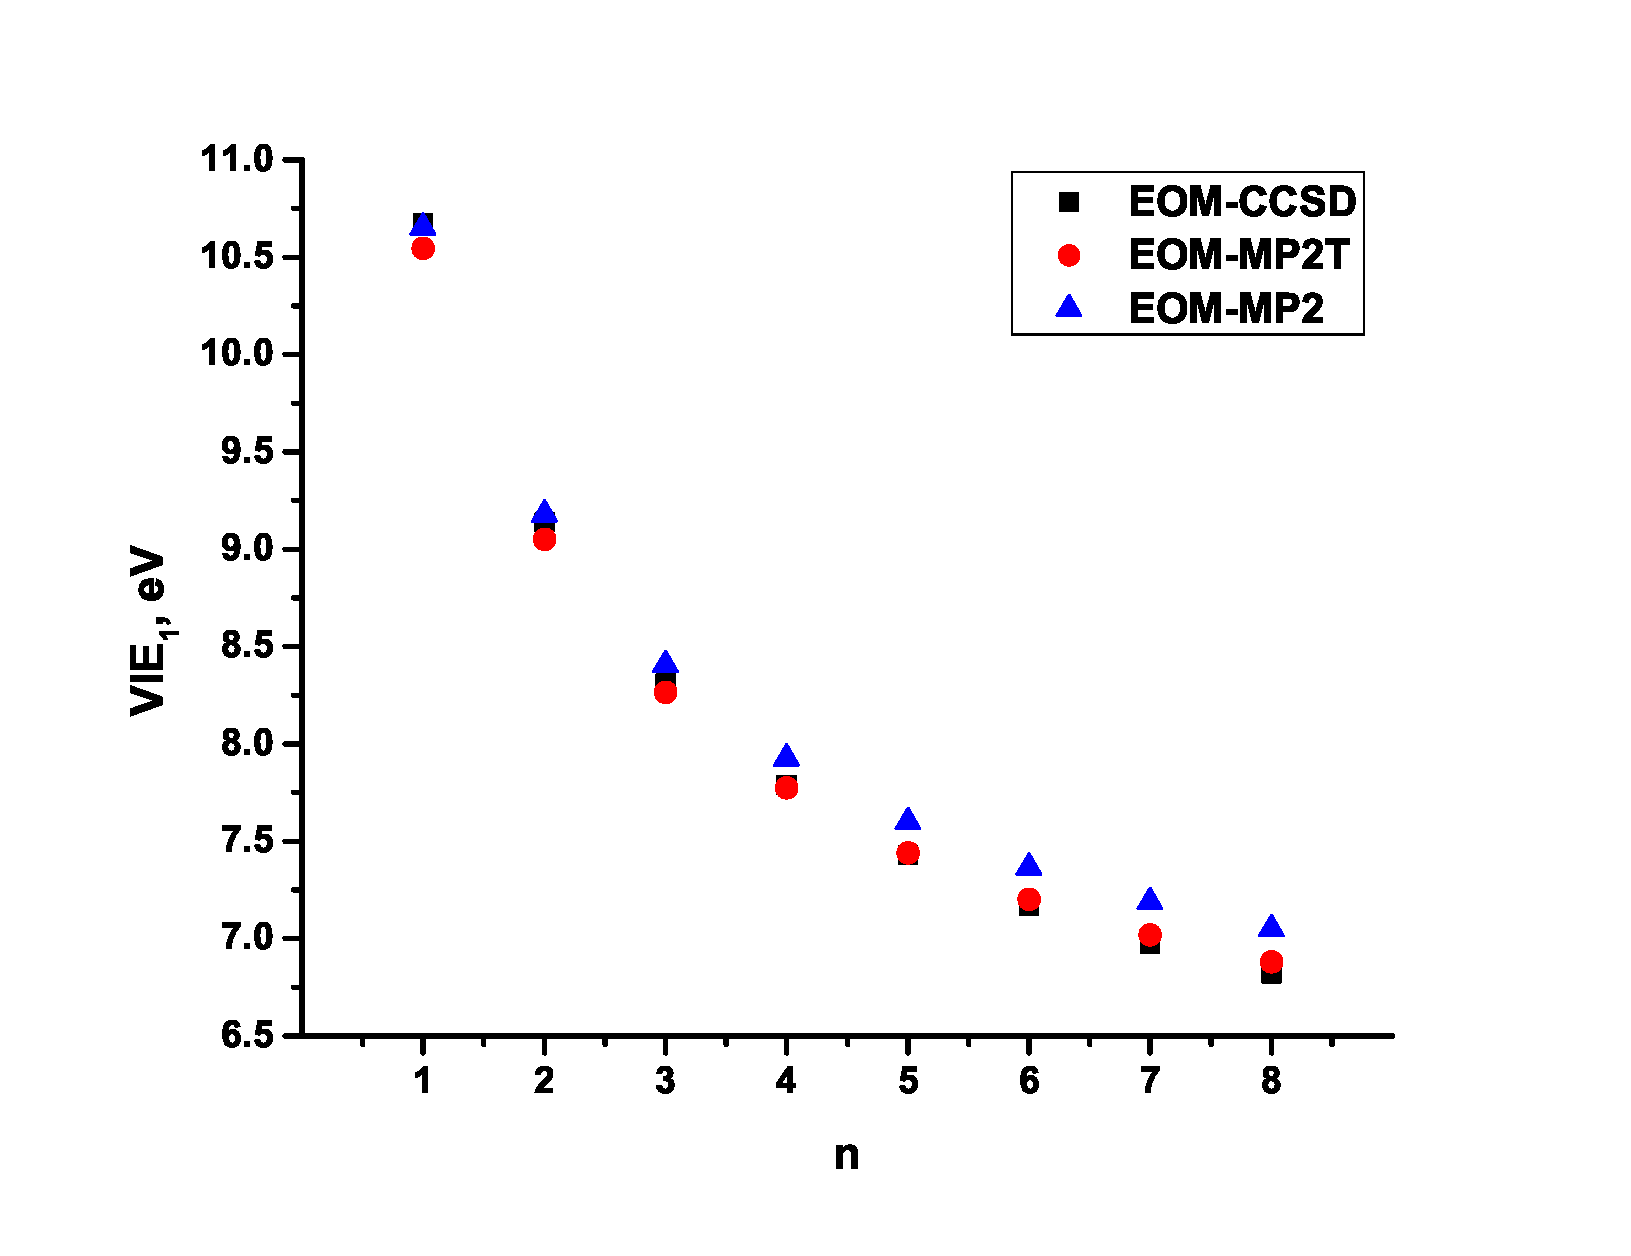
\includegraphics[width=10.5cm]{./figures/size-ext_cc-pVTZ.eps}
	\caption{Size-extensivity numerical test of EOM-MP2T, EOM-CCSD and EOM-MP2 methods for C$_{2n}$H$_{(2n+2)}$ $trans$-polyenes. Geometry optimization: RI-MP2/cc-pVTZ; IP calculations: cc-pVTZ.
		\protect\label{fig:size-ext_cc-pVTZ}}
\end{figure}

\begin{figure}[!tbh]
	\includegraphics[width=14cm]{./figures/size-ext_6-31Gdp.eps}
    %\includegraphics[width=14cm]{./figures/size-ext_6-31Gdp.pdf}
	\caption{Size-extensivity numerical test of EOM-MP2T, EOM-CCSD and EOM-MP2 methods for C$_{2n}$H$_{(2n+2)}$ $trans$-polyenes. Geometry optimization: RI-MP2/6-31G**; IP calculations: 6-31G**.
		\protect\label{fig:size-ext_6-31Gdp}}
\end{figure}

% Table generated by Excel2LaTeX from sheet 'IP'
\begin{table}[!htbp]
  \centering
  \caption{EOM-MP2T, EOM-MP2 and EOM-CCSD vertical ionization energies (eV) of nucleobases, HBDI$^{-}$ chromophore, and nitrogenous base dimers computed with aug-cc-pVTZ (left) and cc-pVTZ (right) bases. (C): Cholesky decomposition of two-electron integrals.}
    \begin{tabular}{c|ccccc|c|c|cccccc}
    \hline\hline
    \textbf{Uracil}  &       &       & orbital № &       &       &       &   \textbf{HBDI$^{-}$}  &       &       & orbital № &       &       &   \\
     & 29    & 27    & 28    & 26    & 25    &       &  & 57    & 54    & 56    & 55    & 53    & 52 \\
        \hline
    EOM-CCSD & 9.67  & 10.35 & 10.74 & 11.30 & 13.19 &       & EOM-CCSD & 2.62  & 4.49  & 4.85  & 5.43  & 6.33  & - \\
    EOM-MP2T & 9.73  & 10.42 & 10.86 & 11.38 & 13.22 &       & EOM-CCSD (C) & 2.62  & 4.49  & 4.85  & 5.43  & 6.33  & - \\
    EOM-MP2 & 9.92  & 10.45 & 10.97 & 11.40 & 13.42 &       & EOM-MP2T & 2.88  & 4.54  & 5.04  & 5.50  & -     & 5.71 \\
          &       &       &       &       &       &       & EOM-MP2 & 3.06  & 4.56  & 5.19  & 5.68  & -     & 5.83 \\
    \hline
    \textbf{Cytosine}  &       &       & orbital № &       &       &     & \textbf{A=T WC}  &       &       & orbital № &       &       &     \\ 
    & 29    & 28    & 27    & 26    & 25    &  &  & 68    & 67    & 65    & 66    & 62    & \\
    \hline
    EOM-CCSD & 8.90  & 9.66  & 9.76  & 10.16 & 12.38 &  &  EOM-CCSD & 8.05  & 8.88  & 9.25  & 9.47  & 9.90  &     \\
    EOM-MP2T & 9.01  & 9.73  & 9.83  & 10.21 & 12.43 &       & EOM-CCSD (C) & 8.05  & 8.89  & 9.25  & 9.47  & 9.90  &   \\
    EOM-MP2 & 9.13  & 9.91  & 9.81  & 10.29 & 12.55 & .& EOM-MP2T & 8.21  & 8.96  & 9.34  & 9.65  & 9.98  &        \\
          &       &       &       &       &       &   & EOM-MP2 & 8.34  & 9.17  & 9.48  & 9.78  & 10.05 &      \\
    \hline
    \textbf{Thymine}         &       &       & orbital № &       &       &  & \textbf{G$\equiv$C WC}  &       &       & orbital № &       &       &     \\
    & 33    & 31    & 32    & 30    & 29  &   & & 68    & 67    & 63    & 66    & 61    &  \\
    \hline
    EOM-CCSD & 9.24  & 10.24 & 10.64 & 11.14 & 12.79 & & EOM-CCSD & 7.35  & 9.23  & 9.27  & 9.37  & 9.55  &        \\
    EOM-MP2T & 9.31  & 10.33 & 10.75 & 11.23 & 12.82 &  & EOM-CCSD (C) & 7.35  & 9.23  & 9.27  & 9.37  & 9.55  &        \\
    EOM-MP2 & 9.51  & 10.36 & 10.87 & 11.25 & 12.99 &   & EOM-MP2T & 7.51  & 9.32  & 9.35  & 9.46  & 9.63  &      \\
          &       &       &       &       &       &      & EOM-MP2 & 7.68  & 9.48  & 9.45  & 9.62  & 9.74  &  \\
    \hline
    \textbf{Adenine}  &       &       & orbital № &       &       &     &\textbf{T-T ST1}  &       &       & orbital № &       &       &       \\
    & 35    & 33    & 34    & 31    & 32    &     &  & 66    & 65    & 62    & 61    & 64    & 63 \\   
    \hline
    EOM-CCSD & 8.44  & 9.45  & 9.71  & 10.50 & 10.68 &       &       EOM-CCSD & 8.88  & 9.26  & 10.12 & 10.16 & 10.40 & -  \\
    EOM-MP2T & 8.62  & 9.54  & 9.91  & 10.58 & 10.82 &  & EOM-CCSD (C) & 8.88  & 9.26  & 10.12 & 10.16 & 10.40 & - \\
    EOM-MP2 & 8.75  & 9.66  & 10.03 & 10.69 & 10.92 &  
    & EOM-MP2T & 8.96  & 9.33  & 10.20 & -     & 10.51 & 10.64  \\
    &&&&&& & EOM-MP2 & 9.19  & 9.56  & 10.28 & 10.32 & 10.68 & - \\
    \hline
    \textbf{Guanine}  &       &       & orbital № &       &       &         &       &       &       &       &       &       &     \\ 
    & 39    & 37    & 35    & 38    & 36    & &       &       &       &       &       &       &               \\
    \hline
    EOM-CCSD & 8.17  & 9.88  & 10.14 & 10.35 & 10.63 & &       &       &       &       &       &       &              \\
    EOM-MP2T & 8.35  & 9.96  & 10.23 & 10.51 & 10.74 &       &       &       &       &       &       &       &  \\
    EOM-MP2 & 8.50  & 10.00 & 10.33 & 10.65 & 10.87 &       &       &       &       &       &       &       &  \\
    \hline\hline
    \end{tabular}%
  \label{tab:eom-ip-values}%
\end{table}%

% Table generated by Excel2LaTeX from sheet 'Errors'
\begin{table}[!htbp]
  \centering
  \caption{Errors and standard deviations (eV) with respect to the EOM-CCSD values for nucleobases.}
    \begin{tabular}{c|ccccc|cc}
    \toprule
    \textbf{Uracil} &  &&Orbital&&       & MUE   & SD \\
          & 29    & 27    & 28    & 26    & 25    &       &  \\
          \hline
    EOM-MP2T & 0.07  & 0.08  & 0.11  & 0.08  & 0.03  & 0.07  & 0.03 \\
    EOM-MP2 & 0.26  & 0.10  & 0.22  & 0.11  & 0.23  & 0.18  & 0.07 \\
    \hline
    \textbf{Cytosine} & &&Orbital&&          & MUE   & SD \\
          & 29    & 28    & 27    & 26    & 25    &       &  \\
          \hline
    EOM-MP2T & 0.12  & 0.07  & 0.07  & 0.04  & 0.05  & 0.07  & 0.03 \\
    EOM-MP2 & 0.24  & 0.25  & 0.05  & 0.12  & 0.17  & 0.17  & 0.08 \\
    \hline
    \textbf{Thymine} &&&Orbital&&           & MUE   & SD \\
          & 33    & 31    & 32    & 30    & 29    &       &  \\
          \hline
    EOM-MP2T & 0.07  & 0.08  & 0.12  & 0.08  & 0.03  & 0.08  & 0.03 \\
    EOM-MP2 & 0.27  & 0.12  & 0.23  & 0.11  & 0.20  & 0.19  & 0.07 \\
    \hline
    \textbf{Adenine} &&&Orbital&&        & MUE   & SD\\
          & 35    & 33    & 34    & 31    & 32    &       &  \\
    \hline
    EOM-MP2T & 0.18  & 0.09  & 0.20  & 0.08  & 0.14  & 0.14  & 0.05 \\
    EOM-MP2 & 0.31  & 0.22  & 0.32  & 0.20  & 0.24  & 0.25  & 0.05 \\
    \hline
    \textbf{Guanine} & &&Orbital&&           &       MUE   & SD   \\
          & 39    & 37    & 35    & 38    & 36    & & \\
    \hline
    EOM-MP2T & 0.18  & 0.08  & 0.08  & 0.16  & 0.11  & 0.12  & 0.04 \\
    EOM-MP2 & 0.33  & 0.12  & 0.19  & 0.30  & 0.24  & 0.23  & 0.09 \\
    \hline\hline
    \end{tabular}%
  \label{tab:errors-nucleobases}%
\end{table}%

% Table generated by Excel2LaTeX from sheet 'Errors'
\begin{table}[!htbp]
  \centering
  \caption{Errors and standard deviations (eV) with respect to the EOM-CCSD values for HBDI$^{-}$ and nitrogenous base dimers.}
    \begin{tabular}{c|ccccc|cc}
    \toprule
    \textbf{HBDI$^{-}$} &       &       & Orbital &       &       & MUE   & SD \\
          & 57    & 54    & 56    & 55    & 53    &       &  \\
          \hline
    EOM-MP2T & 0.26  & 0.05  & 0.19  & 0.08  & -     & 0.14  & 0.10 \\
    EOM-MP2 & 0.44  & 0.08  & 0.34  & 0.26  & -     & 0.28  & 0.15 \\
     \hline
    \textbf{A=T WC} &       &       & Orbital &       &       & MUE   & SD \\
          & 68    & 67    & 65    & 66    & 62    &       &  \\
          \hline
    EOM-MP2T & 0.17  & 0.07  & 0.09  & 0.18  & 0.09  & 0.12  & 0.05 \\
    EOM-MP2 & 0.30  & 0.29  & 0.23  & 0.31  & 0.15  & 0.26  & 0.07 \\
       \hline
    \textbf{G$\equiv$C WC} &       &       & Orbital &       &       & MUE   & SD \\
          & 68    & 67    & 63    & 66    & 61    &       &  \\
          \hline
    EOM-MP2T & 0.16  & 0.10  & 0.08  & 0.09  & 0.09  & 0.10  & 0.04 \\
    EOM-MP2 & 0.33  & 0.25  & 0.18  & 0.24  & 0.19  & 0.24  & 0.06 \\
    \hline
    \textbf{T-T ST1} &       &       & Orbital &       &       & MUE   & SD \\
          & 66    & 65    & 62    & 61    & 64    &       &  \\
    \hline
    EOM-MP2T & 0.08  & 0.07  & 0.08  & -     & 0.11  & 0.08  & 0.02 \\
    EOM-MP2 & 0.32  & 0.30  & 0.16  &  0.16  & 0.28  & 0.24  & 0.08 \\
    \hline\hline
    \end{tabular}%
  \label{tab:hbdi-dimers}%
\end{table}%

\begin{table}[!htbp]
  \centering
  \caption{Wall and CPU timings (h) of EOM-MP2T, EOM-MP2 and EOM-CCSD methods used for calculation of five lowest ionization energies of HBDI$^{-}$ chromophore and nitrogenous base dimers. (C): Cholesky decomposition of two-electron integrals.}
    \begin{tabular}{c|cc}
    \toprule
    \textbf{HBDI$^{-}$} & Wall  & CPU \\
    \hline
    EOM-CCSD & 61    & 209 \\
    EOM-CCSD (C)  & 25    & 312 \\
    EOM-MP2T & 13    & 47 \\
    EOM-MP2 & 13    & 47 \\
    \hline
    \textbf{A=T WC} &       &  \\
    \hline
    EOM-CCSD & 117   & 423 \\
    EOM-CCSD (C)  & 54    & 627 \\
    EOM-MP2T & 25    & 84 \\
    EOM-MP2 & 25    & 79 \\
    \hline
    \textbf{G$\equiv$C WC} &       &  \\
    \hline
    EOM-CCSD & 117   & 391 \\
    EOM-CCSD (C)  & 48    & 542 \\
    EOM-MP2T & 24    & 81 \\
    EOM-MP2 & 24    & 81 \\
    \hline
    \textbf{T-T ST1} &       &  \\
    \hline
    EOM-CCSD & 77    & 323 \\
    EOM-CCSD (C)  & 37    & 474 \\
    EOM-MP2T & 23    & 96 \\
    EOM-MP2 & 23    & 96 \\
    \hline\hline
    \end{tabular}%
  \label{tab:addlabel}%
\end{table}%

\clearpage
\section{NEW DATA: SET1 and SET2, EOM-IP/EE/EA-MP2/MP2T/CCSD}
\begin{figure}[!tbh]
	\includegraphics[width=15cm]{./figures/set1.pdf}
	\caption{Set 1.
		\protect\label{fig:set1}}
\end{figure}

\begin{figure}[!tbh]
	\includegraphics[width=15cm]{./figures/set2.pdf}
	\caption{Set 2.
		\protect\label{fig:set2}}
\end{figure}

\clearpage
% Table generated by Excel2LaTeX from sheet 'set1_IP_nucleobases'
\begin{table}[htbp]
	\centering
	\caption{Mean signed and unsigned errors (MSE, MUE), standard deviation (SD), and maximum unsigned error in ionization energies of molecules in set 1 with respect to EOM-CCSD.}
	\begin{tabular}{ccc}
		\toprule
		& EOM-MP2 & EOM-MP2T \\
		\hline
		MSE   & 0.239 & 0.103 \\
		MUE   & 0.239 & 0.103 \\
		SD    & 0.078 & 0.045 \\
		Max. UE & 0.367 & 0.206 \\
		\hline
	\end{tabular}%
	\label{tab:set1_ip}%
\end{table}%


% Table generated by Excel2LaTeX from sheet 'set1_EE_nucleobases'
\begin{table}[htbp]
	\centering
	\caption{Mean signed and unsigned errors (MSE, MUE), standard deviation (SD), and maximum unsigned error in excitation energies of molecules in set 1 with respect to EOM-CCSD.}
	\begin{tabular}{ccc}
		\toprule
		& EOM-MP2 & EOM-MP2T \\
		\hline
		MSE   & 0.211 & 0.175 \\
		MUE   & 0.211 & 0.175 \\
		SD    & 0.105 & 0.072 \\
		Max. UE & 0.385 & 0.327 \\
		\hline
	\end{tabular}%
	\label{tab:set1_ee}%
\end{table}%


% Table generated by Excel2LaTeX from sheet 'set1_EA_nucleobases'
\begin{table}[htbp]
	\centering
	\caption{Mean signed and unsigned errors (MSE, MUE), standard deviation (SD), and maximum unsigned error in electron attachment energies of molecules in set 1 with respect to EOM-CCSD.}
	\begin{tabular}{ccc}
		\toprule
		& EOM-MP2 & EOM-MP2T \\
		\hline
		MSE   & -0.003 & 0.051 \\
		MUE   & 0.044 & 0.058 \\
		SD    & 0.053 & 0.063 \\
		Max. UE & 0.112 & 0.155 \\
		\hline
	\end{tabular}%
	\label{tab:set1_ea}%
\end{table}%


% Table generated by Excel2LaTeX from sheet 'set2_other_bio_IP'
\begin{table}[htbp]
	\centering
	\caption{Mean signed and unsigned errors (MSE, MUE), standard deviation (SD), and maximum unsigned error in ionization energies of molecules in set 2 with respect to EOM-CCSD.}
	\begin{tabular}{ccc}
		\toprule
		& EOM-MP2 & EOM-MP2T \\
		\hline
		MSE   & 0.237 & 0.088 \\
		MUE   & 0.237 & 0.093 \\
		SD    & 0.099 & 0.081 \\
		Max. UE & 0.473 & 0.262 \\
		\hline
	\end{tabular}%
	\label{tab:set2_ip}%
\end{table}%


% Table generated by Excel2LaTeX from sheet 'set2_other_bio_EE'
\begin{table}[htbp]
	\centering
	\caption{Mean signed and unsigned errors (MSE, MUE), standard deviation (SD), and maximum unsigned error in excitation energies of molecules in set 2 with respect to EOM-CCSD.}
	\begin{tabular}{ccc}
		\toprule
		& EOM-MP2 & EOM-MP2T \\
		\hline
		MSE   & 0.224 & 0.161 \\
		MUE   & 0.224 & 0.161 \\
		SD    & 0.057 & 0.078 \\
		Max. UE & 0.357 & 0.348 \\
		\hline
	\end{tabular}%
	\label{tab:set2_ee}%
\end{table}%


% Table generated by Excel2LaTeX from sheet 'set2_other_bio_EA'
\begin{table}[htbp]
	\centering
	\caption{Mean signed and unsigned errors (MSE, MUE), standard deviation (SD), and maximum unsigned error in electron attachment energies of molecules in set 2 with respect to EOM-CCSD.}
	\begin{tabular}{ccc}
		\toprule
		& EOM-MP2 & EOM-MP2T \\
		\hline
		MSE   & -0.001 & 0.037 \\
		MUE   & 0.026 & 0.051 \\
		SD    & 0.037 & 0.056 \\
		Max. UE & 0.100 & 0.156 \\
		\hline
	\end{tabular}%
	\label{tab:set2_ea}%
\end{table}%

\bibliographystyle{jacs_full}
\bibliography{abbr,kbravaya,dg,ab_initio,rtazhigulov-refined,krylovgroup,vm}
\end{document}
